%% Creator: Inkscape inkscape 0.92.1, www.inkscape.org
%% PDF/EPS/PS + LaTeX output extension by Johan Engelen, 2010
%% Accompanies image file 'Wavelet_Haar.pdf' (pdf, eps, ps)
%%
%% To include the image in your LaTeX document, write
%%   \input{<filename>.pdf_tex}
%%  instead of
%%   \includegraphics{<filename>.pdf}
%% To scale the image, write
%%   \def\svgwidth{<desired width>}
%%   \input{<filename>.pdf_tex}
%%  instead of
%%   \includegraphics[width=<desired width>]{<filename>.pdf}
%%
%% Images with a different path to the parent latex file can
%% be accessed with the `import' package (which may need to be
%% installed) using
%%   \usepackage{import}
%% in the preamble, and then including the image with
%%   \import{<path to file>}{<filename>.pdf_tex}
%% Alternatively, one can specify
%%   \graphicspath{{<path to file>/}}
%% 
%% For more information, please see info/svg-inkscape on CTAN:
%%   http://tug.ctan.org/tex-archive/info/svg-inkscape
%%
\begingroup%
  \makeatletter%
  \providecommand\color[2][]{%
    \errmessage{(Inkscape) Color is used for the text in Inkscape, but the package 'color.sty' is not loaded}%
    \renewcommand\color[2][]{}%
  }%
  \providecommand\transparent[1]{%
    \errmessage{(Inkscape) Transparency is used (non-zero) for the text in Inkscape, but the package 'transparent.sty' is not loaded}%
    \renewcommand\transparent[1]{}%
  }%
  \providecommand\rotatebox[2]{#2}%
  \ifx\svgwidth\undefined%
    \setlength{\unitlength}{407.96159363bp}%
    \ifx\svgscale\undefined%
      \relax%
    \else%
      \setlength{\unitlength}{\unitlength * \real{\svgscale}}%
    \fi%
  \else%
    \setlength{\unitlength}{\svgwidth}%
  \fi%
  \global\let\svgwidth\undefined%
  \global\let\svgscale\undefined%
  \makeatother%
  \begin{picture}(1,0.2299448)%
    \put(0,0){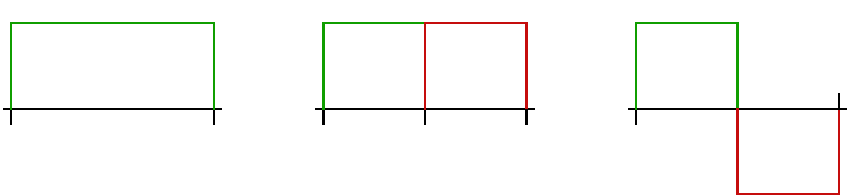
\includegraphics[width=\unitlength,page=1]{Wavelet_Haar.pdf}}%
    \put(0.7960309,0.1700815){\color[rgb]{0,0,0}\makebox(0,0)[lb]{\smash{}}}%
    \put(0.01282578,0.05882918){\color[rgb]{0,0,0}\makebox(0,0)[b]{\smash{$0$}}}%
    \put(0.25181801,0.05882918){\color[rgb]{0,0,0}\makebox(0,0)[b]{\smash{$1$}}}%
    \put(0.13232146,0.14004219){\color[rgb]{0,0,0}\makebox(0,0)[b]{\smash{$\phi(t)$}}}%
    \put(0.3805066,0.05882918){\color[rgb]{0,0,0}\makebox(0,0)[b]{\smash{$0$}}}%
    \put(0.50000315,0.05882918){\color[rgb]{0,0,0}\makebox(0,0)[b]{\smash{$0.5$}}}%
    \put(0.44025398,0.14004219){\color[rgb]{0,0,0}\makebox(0,0)[b]{\smash{$\phi(2t)$}}}%
    \put(0.55975137,0.14004219){\color[rgb]{0,0,0}\makebox(0,0)[b]{\smash{$\phi(2t-1)$}}}%
    \put(0.61949976,0.05882918){\color[rgb]{0,0,0}\makebox(0,0)[b]{\smash{$1$}}}%
    \put(0.74818835,0.05882918){\color[rgb]{0,0,0}\makebox(0,0)[b]{\smash{$0$}}}%
    \put(0.86455027,0.07867825){\color[rgb]{0,0,0}\makebox(0,0)[rb]{\smash{$0.5$}}}%
    \put(0.80793567,0.14004219){\color[rgb]{0,0,0}\makebox(0,0)[b]{\smash{$\phi(2t)$}}}%
    \put(0.92743306,0.03892961){\color[rgb]{0,0,0}\makebox(0,0)[b]{\smash{$-\phi(2t-1)$}}}%
    \put(0.98718145,0.13130257){\color[rgb]{0,0,0}\makebox(0,0)[b]{\smash{$1$}}}%
    \put(0.86768586,0.21877072){\color[rgb]{0,0,0}\makebox(0,0)[b]{\smash{$\psi(t)$}}}%
  \end{picture}%
\endgroup%
